% !TEX encoding = UTF-8
% !TEX TS-program = pdflatex
% !TEX root = ../Tesi.tex
% !TEX spellcheck = it-IT

%************************************************

%************************************************

Il progressivo aumento della dimensione del Web e le informazioni in esso contenute fanno di esso la più grande sorgente informativa pubblicamente accessibile. Il Web infatti contiene qualsiasi tipo di informazione in qualsiasi tipo di formato. 
La sua grande eterogeneità rende l'estrazione e il reperimento delle informazioni un task altamente complesso. 
% il più grande insieme di dati da cui poter estrarre informazione velocemente e liberamente. Il Web è la sorgente informativa più eterogenea tra quelle esistenti, data la sua natura, e contenente dati prevalentemente non strutturati o semi-strutturati. Il problema non è sapere se le informazioni ci sono, ma riuscire a trovarle. 

Sebbene a prima vista il Web possa sembrare un insieme disordinato e non strutturato di informazioni distribuite su molteplici pagine web, in realtà è possibile estrarre molteplici correlazioni nascoste tra informazioni all'interno della stessa pagina web e informazioni tra pagine web connesse tramite hyperlink.

%Anche se a prima vista il Web sembra un insieme disordinato di pagine senza nessuna correlazione logica nella struttura, sia interna che nelle relazioni tra queste, in realtà possono essere trovate numerose correlazioni  nascoste. 
Riuscire ad estrarre tali correlazioni e pattern, analizzando la struttura ad hyperlink di cui il Web si compone, permetterebbe di migliorare diverse applicazioni esistenti.

Il problema rimane l'individuazione del procedimento adatto al compito prefissato. Tecniche e metodologie per l'estrazione di conoscenza da grandi quantità di dati sono già state sviluppate nell'area del Data Mining. Trasferire questo sapere nel Web, tuttavia, può non essere semplice e immediato, date la caratteristiche che lo contraddistinguono. 
Di seguito sarà introdotto il contesto in cui si sviluppa la tesi, le varie aree in cui si colloca e da cui attinge le metodologie ed il bagaglio di conoscenza utile alla sintesi di nuovi algoritmi di estrazione di conoscenza dal Web.

\section{Data Mining nel Web}
Il Data Mining è l'insieme di tecniche e metodologie che hanno per oggetto estrazione di informazione utile, di un sapere o di una conoscenza a partire da grandi quantità di dati.

Il concetto di informazione è strettamente legato al contesto in cui si esegue un task di apprendimento, in altre parole un dato può essere interessante o trascurabile a seconda del tipo di applicazione in cui si vuole operare. La fase di estrazione di informazione dai dati per renderla direttamente utilizzabile può variare enormemente dal dominio applicativo. Le differenze sono tali da dover suddividere tali procedimenti in aree diverse, dipendenti dal tipo di dati da cui parte il processo di estrazione. Principalmente le grandi moli di dati possono variare da grandi collezioni di documenti, database, pagine Web ecc, differenziandosi molto nella struttura e nel contenuto,.
\\\\
Il \textbf{Web Mining} è l’applicazione delle tecniche di Data Mining per la scoperta e l’estrazione di conoscenza o di pattern dal World Wide Web.
\\
Le proprietà che caratterizzano il Web e che lo differenziano da altre sorgenti di dati sono:
\begin{itemize}
\item \textbf{Dimensione}: 

Il Web è il primo mezzo di informazione dove il numero di produttori di informazioni è uguale al numero dei consumatori. La quantità dei dati da processare può essere più grande di svariati ordini di grandezza rispetto a tradizionali task di Data Mining. Diventa necessario l'utilizzo di tecniche scalabili, ossia la capacità di un sistema di ''crescere'' ed essere utilizzabile in funzione della crescita dei dati. Nel Data Mining tradizionale, processare un milione di record può essere considerato sopra la media, mentre nel Web Mining dieci milioni di pagine possono non essere abbastanza. 

\item \textbf{Dinamicità}: 
Ogni secondo migliaia sono create, distrutte e modificate migliaia di pagine Web. Questo rende il Web una rete di informazioni dinamica, dove la struttura e il contenuto dell'informazione cambiano frequentemente. Monitorare questi cambiamenti rimane un problema importante per molte applicazioni.

\item \textbf{Eterogeneità}:
L'eterogeneità del Web dipende sia dal formato delle pagine che dalla scrittura. Nel primo caso, l'eterogeneità è dovuta al fatto che nel Web non esiste uno standard di formato per le pagine Web che possono ricadere in tre categorie: \textit{i)}pagine non strutturate \textit{ii)} pagine strutturate \textit{iii)} pagine semi-strutturate.
\\
Le pagine \textit{non strutturate}, anche chiamate \textit{free-text pages}, sono scritte in linguaggio naturale e possono essere applicate tecniche con un certo grado di affidabilità.
\\
Le pagine \textit{strutturate} sono normalmente ottenute da sorgenti di dati strutturate (e.g. database). Le tecninche di estrazione sono applicate usando l'individuazione di regole sintattiche.
Le pagine \textit{semi-strutturate} si posizionano al centro delle precedenti. Possiedono infatti un certo livello di struttura, nascosto nel testo. L'estrazione può avvenire cercando pattern nei tag HTML.
\\
In questo caso l'eterogeneità è dovuta al fatto che le pagine Web son create da milioni di persone aventi differente cultura, abilità, linguaggio, ecc. Questo significa che le pagine potrebbero contenere la stessa informazione, ma presentata in maniera completamente diversa. Questo rende il processo di estrazione dell'informazione una sfida.

\item \textbf{Connessione}: Il web è generalmente rappresentato come una rete di informazioni dove i nodi sono le pagine e gli archi sono gli hyperlink. Gli hyperlink fra le pagine di uno stesso sito e quelli fra le pagine di siti diversi, hanno diverse caratteristiche e funzionalità. All'interno di un sito servono ad organizzare i contenuti, mentre fra siti diversi servono a trasportare autorità alla pagina di destinazione. In questo caso significa che come persone ci fidiamo del contenuto di queste pagine.

\item \textbf{Rumore}: 
Differentemente da altri mezzi di informazione, la pubblicazione di contenuti è libera e non richiede approvazione. Questo contribuisce all'aumentare del volume e della diversità dell'informazione, ma anche

\item \textbf{Società virtuale}: Il web è generalmente rappresentato come una rete di informazioni dove i nodi sono le pagine e gli archi sono gli hyperlink. Gli hyperlink fra le pagine di uno stesso sito e quelli fra le pagine di siti diversi, hanno diverse caratteristiche e funzionalità. All'interno di un sito servono ad organizzare i contenuti, mentre fra siti diversi servono a trasportare autorità alla pagina di destinazione. In questo caso significa che come persone ci fidiamo del contenuto di queste pagine.

\end{itemize}

Sulla base di queste, task di Web Mining possono utilizzare tecniche diverse ed essere finalizzate alla scoperta di informazioni differenti. Si possono distinguere principalmente tre categorie:
\begin{itemize}
\item \textit{Web Usage Mining}, è l’applicazione di tecniche di Data Mining per la scoperta di pattern e informazioni utili attraverso l'analisi di log immagazzinati dai web server e contenenti click stream. 
Obiettivo di questo campo è l'apprendimento dell'identità, origine e comportamenti degli utenti che navigano i siti web al fine di comprendere i loro bisogni e ad offrire loro servizi migliori attraverso una personalizzazione dell'esperienza web.
\item \textit{Web Structure Mining}, consiste nell'estrazione di relazioni sconosciute o nascoste tra pagine web attraverso l'analisi della struttura ad hyperlink di un sito web (anche chiamato ``grafo web''). Questo task verrà analizzato in dettaglio nella Sezione \ref{subsec:webstructure}.
\item \textit{Web Content Mining}, consiste nell'estrazione ed integrazione di informazione utile e precedentemente sconosciuta dal contenuto delle pagine web. Ricadono in questo campo due principali tipologie di algoritmi: \textit{i)} algoritmi capaci di raggruppare e classificare pagine web in funzione del loro contenuto testuale o del topic descritto; \textit{ii)} algoritmi per estrarre pattern strutturati contenuti nelle pagine web (per esempio liste di prodotti commerciali, professori, etc.).  
Sebbene questi algoritmi possano sembrare molto simili ai più famosi algoritmi di Data Mining e Text Mining, le pagine web hanno delle proprietà e peculiarità che rendono tali algoritmi non direttamente applicabili. Un'importante branca del Web Content Mining è rappresentato dal Web Information Extraction, il cui obiettivo è quello di estrarre dati strutturati da pagine web e integrarli in tabelle relazionali. In questo contesto il Web Content Mining può essere visto quindi come reperimento e immagazzinamento di informazioni.
\end{itemize}



\color{black}

STAI PARLANDO DI 3 COSA DIVERSE E LE STAI METTENDO NELLO STESSO CALDERONE (DIFFERENZE DATA MINING E WEB MINING, CARATTERISTICHE DEL WEB, PRESENZA DI DATI STRUTTURATI E NON STRUTTURATI)
SISTEMALI IN MODO CHE ESCA UN DISCORSO OMOGENEO E FLUENTE
\color{red}

Enormi sforzi son stati fatti per combinare informazione strutturata e non strutturata presente all'interno di pagine web, al fine di estrarre, indicizzare e reperire nuova conoscenza. 
La maggior parte delle soluzioni attuali trasformano il contenuto testuale delle pagine web in uno spazio vettoriale \cite{Turney10}. Modelli basati su spazi vettoriali sono fondamentali per task che coinvolgono il calcolo della similarità tra oggetti in cui oggetti simili sono caratterizzati da rappresentazioni vettoriali simili. Il modello vettoriale \textit{termini-documenti} rappresenta il più semplice e utilizzato modello di rappresentazione di documenti testuali nel contesto del Text Mining. In tale modello il valore dell'elemento $i$-esimo in un vettore documento rappresenta il numero di volte che il termine $i$ compare nel documento stesso.    
Gli algoritmi basati su modelli di rappresentazione vettoriali si basano sull'assunzione di indipendenza tra i termini all'interno di un documento e tra i documenti stessi. Le pagine web violano come tutti i documenti testuali la prima assunzione, inoltre i collegamenti ipertestuali definendo relazioni di interdipendenza tra le pagine stesse comportano la violazione della seconda assunzione.

Di conseguenza gli algoritmi di Web Mining devono tener conto delle informazioni relative alla struttura del sito web a cui appartengono al fine di estrarre informazioni più accurate.
\color{black}
\section{Web Structure mining}
\label{subsec:webstructure}
Un enorme quantità di informazioni dal web sono rappresentati come dati semi-strutturati, ossia come combinazione di testo non strutturato e dati strutturati. I dati strutturati contenuti nelle pagine web sono tipicamente dati generati dinamicamente dalla struttura sottostante, come un database relazionale, o da un template statico.
\\\\
Estrarre questi dati è utile in molti domini applicativi perchè permette di ottenere ed integrare dati da diverse fonti, producendo così servizi migliori, informazioni personalizzate, meta-ricerche. Con sempre più aziende ed organizzazioni che disseminano informazioni in rete, l’abilità di estrarre questi dati dalle pagine web sta diventando estremamente importante.
\\\\
Differentemente dai documenti testuali tradizionali, i dati strutturati nelle pagine web sono arricchiti da hyperlink che dividono l’informazione in molteplici ed interdipendenti pagine web. Questi hyperlink possono essere usati per identificare le entità provenienti dal mondo reale (e.g. pagine di professori, corsi, prodotti) e le relazioni che intercorrono fra di esse. Dato che i documenti web non sono nè strutturati come un database nè completamente non-strutturati come documenti testuali, le tecniche tradizionali di data mining o text mining non possono essere applicate direttamente. 
\\\\
Nel primo caso, le tecniche di data mining si basano sul presupposto che i dati usati per apprendere un modello condividono uno schema comune, avente delle tabelle ben definite con attributi, colonne, tuple e vincoli. Le pagine web non hanno questo presupposto perchè contengono dati eterogenei e gli hyperlink definiscono relazioni il cui significato può variare profondamente. Inoltre le pagine web sono codificate in HTML che, differentemente da altri linguaggi di markup, è stato progettato solo per la renderizzazione dei dati. Per questa ragione, il web può essere considerato un moderno legacy system, in quanto una grande quantità di dati non è facilmente accessibile e manipolabile direttamente. 
\\\\
Nel secondo caso, le tecniche di text mining falliscono nell’apprendere modelli accurati perchè richiedono collezioni di documenti scritti in modo consistente e non sono in grado di gestire informazioni complesse con elementi che possiedono diversi ruoli semantici e che forniscono diverse funzionalità. Infatti differentemente dai documenti testuali, le pagine web hanno molteplici rappresentazioni che forniscono differenti informazioni. Una è la rapresentazione testuale del testo HTML, l’altra è la rappresentazione visuale renderizzata da un web browser. Algoritmi di text mining si concentrano sulla rapresentazione testuale ed ignorano la rappresentazione visuale. Di conseguenza, esiste un forte bisogno nel campo dell’informatica di creare approcci e tecniche che usando informazioni testuali, strutturali e visuali sono capaci di estrarre uno schema da dati strutturati ed allineare i dati seguendo tale schema.
\\\\
Il Web Structure Mining può essere diviso in due tipi:
\begin{itemize}
\item Estrazione di dati strutturati tra pagine web attraverso l'analisi del sito web. In questo caso un sito web è rappresentato come un grafo $G = (V, E)$ dove $V$ è l'insieme delle pagine web e $E$ è l'insieme degli hyperlink.
\item Estrazione di dati strutturati contenuti in una pagina web, analizzandone la struttura ad albero basata su tag HTML ed XML.
\end{itemize}
Tra i più importanti algoritmi di web structure mining troviamo Page Rank\cite{} e HITS\cite{}, i quali sfruttano la struttura ad hyperlink del Web per estrarre rank di pagine web.
\color{red}
SCRIVI UN CAPOVERSO QUI IN NODO DA UNIRTI CON LA SEZIONE SUCCESSIVA
\color{black}
\section{Rappresentazioni vettoriali di pagine Web}
La carenza di struttura delle pagine web obbliga all'effettuare dei passaggi preliminari per rendere processabili i dati disponibili. Metodi efficaci consistono nel rappresentare le pagine web come vettori, motivato dal fatto che task di machine learning richiedono input che sono matematicamente e computazionalmente convenienti da elaborare, considerando solo un sottoinsieme significativo dei dati in modo da astrarre ed eliminare informazioni ritenute non pertinenti al risultato finale. Questa fase è probabilmente la più importante in quanto algoritmi di apprendimento tanto bene quanto meglio i vettori ricavati rappresentano bene i dati di partenza. È necessario quindi estrarre rappresentazioni utili dai dati grezzi. Esistono molti modi per ricavare questa correlazione, come reti neurali, matrici di co-occorrenza, dimensionality reduction o rappresentazioni del contesto in cui appare la parola. 
\\\\
L'alternativa proposta in questa tesi consiste nell'utilizzare tecniche di Word Embedding per apprendere rappresentazioni vettoriali dei vertici all'interno del grafo.
Il Word Embedding è il nome di un insieme di tecniche per il language modeling e per il Feature Learning nel campo del Natural Language Processing (NLP)\cite{Bengio03}, utilizzate  in collezioni di documenti, dove ad ogni parola viene associato un vettore detto \textit{Feature Vector}. 
\\\\
Il Word Embedding può essere visto come una funzione parametrizzata 
\begin{equation}
  W : words \to \mathbb{R^n}
\end{equation}
che associa una parola in un dato linguaggio ad un vettore multidimensionale. Un esempio potrebbe essere:
\begin{equation}
  W\left ( "cat" \right ) = \left ( 0.2, -0.4, 0.7, \ldots \right )
\end{equation}
A parole simili corrisponde un vettore simile. Se si cambia una parola con un sinonimo, la validità della frase in esame non cambia (e.g. molti cantano bene $\to$ tanti cantano bene). Questo permette di generalizzare da una frase ad una classe di frasi simili o di capire se una frase è valida, ovvero se  è formulata correttamente.  
\\\\
Questo non significa solo poter scambiare una parola con un sinonimo, ma anche di cambiare una parola con una altra in una classe simile (eg. il muro è rosso → il muro è blu) \cite{Collobert11}. Questo può essere appreso analizzando il contesto della parola da analizzare. Ad esempio ci saranno molti casi in cui sono state osservate frasi valide di questo tipo, quindi cambiando la parola “rosso” con la parola “blu” porterebbe alla creazione una frase ugualmente valida. 
\begin{figure}[htb]
	\centering
	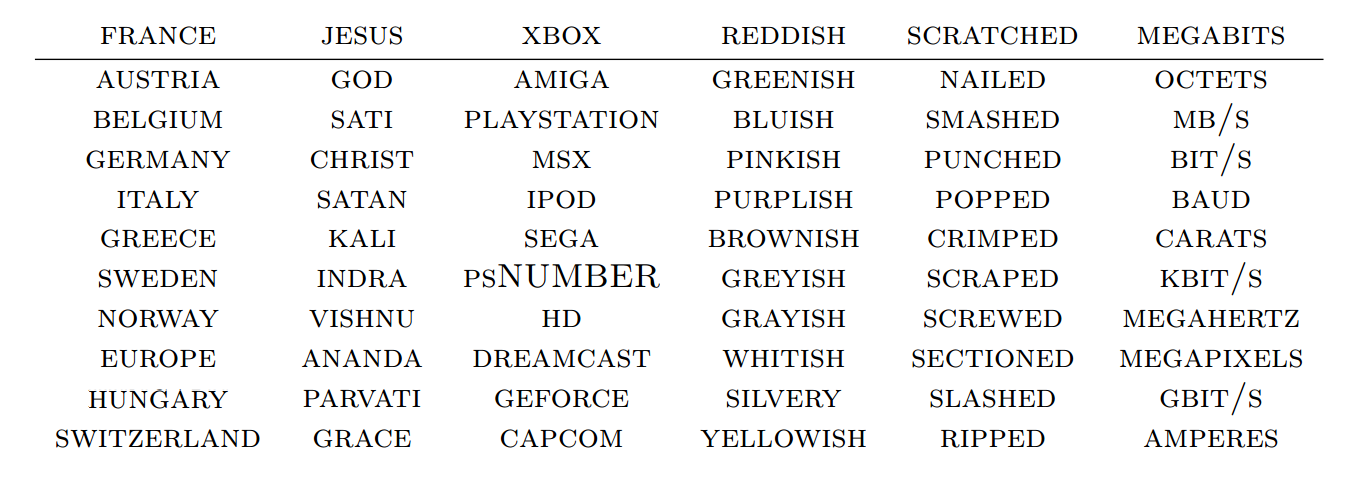
\includegraphics[width = 100mm]{weanalogies.png}
	\caption{Parole con vettori simili}
	\label{similarwords}
\end{figure}

Da questo potrebbe sembrare necessario osservare esempi relativi ad ogni parola per permetterci di generalizzarla. Comprendi tutte le parole che hai già visto, ma non hai già visto tutte le frasi che riesci a capire. Questo è l’approccio delle reti neurali.

\paragraph{Analogie}Il Word Embedding mostra un altra proprietà interessante anche se molto controversa: le analogie. Le analogie tra parole sembrano essere nascoste nella differenza dei loro rispettivi vettori \cite{Mikolov13}. 
\begin{equation}
  W\left ( "woman" \right ) -  W\left ( "man" \right ) \simeq W\left ( "aunt" \right ) -  W\left ( "uncle" \right )
\end{equation}
Da questo si evince che c’è una correlazione tra delle parole e le rispettive forme del genere opposto in quanto appariranno in contesti simile, differenti solo per alcuni dettagli come pronomi o articoli. Stessa cosa per tra singolare e plurale \cite{Mikolov13}.
\begin{figure}[htb]
	\centering
	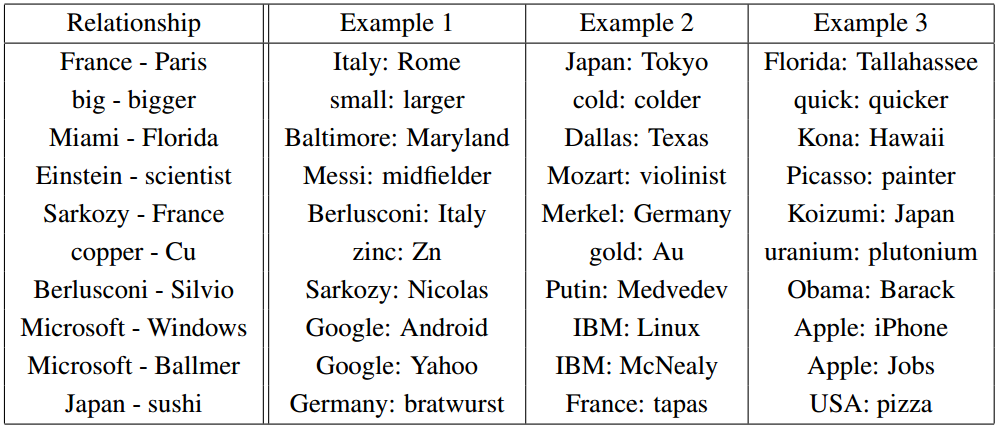
\includegraphics[width = 100mm]{weanalogies2.png}
	\caption{Alcuni esempi di analogie}
	\label{analogies}
\end{figure}
Queste proprietà possono essere considerate effetti collaterali. Non si è cercato di far apprendere il modello in modo da avere parole simili vicine fra loro. Questo sembra essere un punto di forza delle reti neurali nell’apprendere features che rappresentano bene i dati in modo automatico. invece di apprendere un rappresentazione dei dati specifica ed usarla per diversi task, è possibile apprendere un metodo per associare diversi tipi di dati in una singola rappresentazione. Queste tecniche sono note come Transfer Learning, metodi per applicare la conoscenza già appresa in contesti simili.
\\\\
Un esempio può essere il Word Embedding di parole linguaggi diversi. Dato che parole simili saranno associate a vettori simili, parole con significato simile in una lingua e nell’altra finiranno vicine tra loro, così come i loro sinonimi. È possibile notare che anche parole di cui non si conosceva la traduzione o che avessero significati simili, sono finite vicine tra loro \cite{Zou13}.
\begin{figure}[htb]
	\centering
	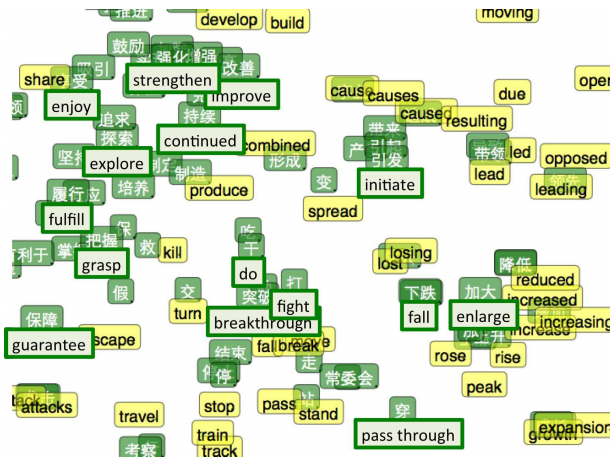
\includegraphics[width = 100mm]{englishchinese.png}
	\caption{Visualizzazione con t-SNE di un Word Embedding bilingua. }
	\label{englishchinese}
\end{figure}


\subsection{Word2vec}
\label{word2vec}
Un algoritmo molto famoso di word embedding è il recente word2vec. L’algoritmo usa i documenti per far apprendere una rete neurale, massimizzando la probabilità condizionata del contesto data una parola, applicando il modello appreso ad ogni parola per ricavare il vettore corrispondente e calcolando il vettore della frase facendo la media dei vettori delle parole, costruisce la matrice di similarità delle frasi ed usa PageRank per classificare le frasi nel grafo.
\begin{equation}
   arg\max_{\theta} \prod_{\left ( w, c \right ) \in D} p\left ( c|w; \theta \right )
\end{equation}
L’obiettivo è di ottimizzare il parametro $ \left (\theta \right )$ massimizzando la probabilità condizionata del contesto $\left ( c \right )$ data la parola $\left ( w \right )$. $D$ è l’insieme di tutte le coppie $\left ( w, c \right )$. 
Per esempio: “ho mangiato un \underline{\hspace{1cm}}  al McDonald ieri sera”, molto probabilmente restituirà “Big Mac”.
\\\\
Applicare il modello di ogni parola per ottenere il suo vettore corrispondente (Figura \ref{2w2v})
\begin{figure}[htb]
	\centering
	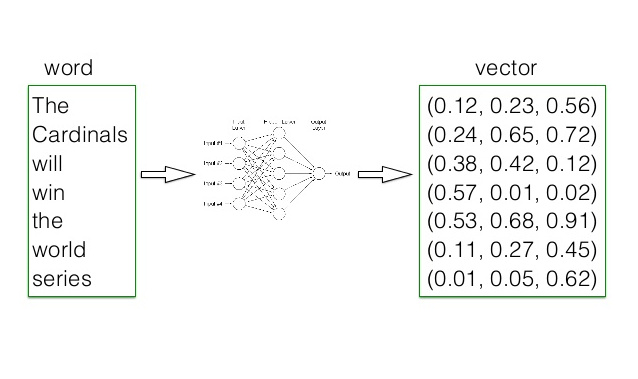
\includegraphics[width = 100mm]{2w2v.jpg}
	\caption{Vettori corrispondenti alle parole}
	\label{2w2v}
\end{figure}
\\\\
Calcolare il vettore delle frasi facendo la media del vettore delle loro parole (Figura \ref{3w2v})
\begin{figure}[htb]
	\centering
	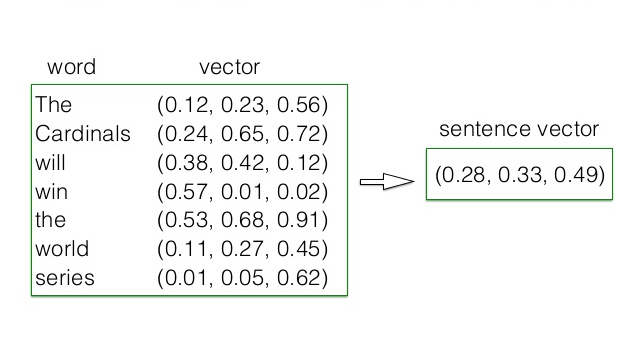
\includegraphics[width = 100mm]{3w2v.jpg}
	\caption{Vettori corrispondenti alle frasi}
	\label{3w2v}
\end{figure}
\\\\
Costruire la matrice di similarità delle frasi (Figura \ref{4w2v})
\begin{figure}[htb]
	\centering
	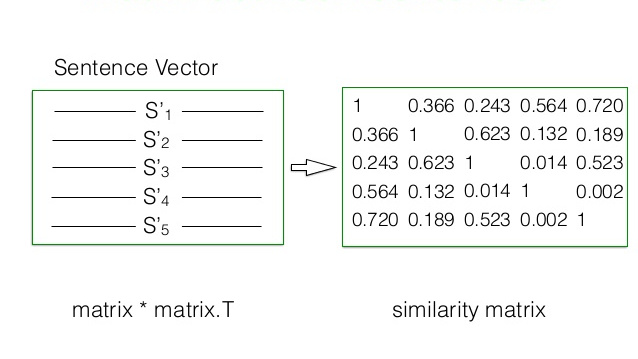
\includegraphics[width = 100mm]{4w2v.jpg}
	\caption{Matrice di similarità}
	\label{4w2v}
\end{figure}
\\\\
Infine usare PageRank par classificare le frasi nel grafo.
 (Figura \ref{5w2v})
\begin{figure}[htb]
	\centering
	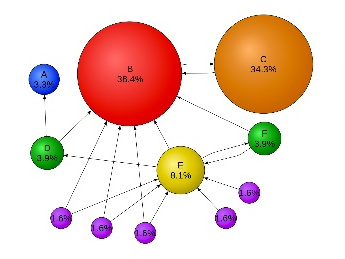
\includegraphics[width = 100mm]{5w2v.jpg}
	\caption{Assegna uno "score" utilizzando Pagerank}
	\label{5w2v}
\end{figure}

Word2vec è una rete neurale a due layer, sebbene non sia profonda (deep neural network) come spesso definita, trasforma il testo in modo che altre reti neurali possano comprenderlo. Prende in input un corpus di documenti e genera un insieme di vettori: feature vectors per ogni parola del corpus. I vettori restituiti sono rappresentazioni numeriche del contesto della singola parola. 
\\\\
Dati abbastanza dati, utilizzo e contesti, word2vec può apprendere rappresentazioni delle parole altamente accurate, basate sulle apparizioni della parola nei diversi contesti. Queste rappresentazioni possono essere usate per trovare associazioni fra parole o per raggruppare documenti e classificarli per argomento. La similarità fra i vettori può essere misurata attraverso la coseno similarità, dove nessuna similarità è espressa come un angolo di 90 gradi, mentre una similarità totale è data  da un angolo di 0 gradi tra i vettori. Ad esempio il vettore relativo a “Sweden” è uguale al vettore “Sweden” mentre il vettore “Norway” ha una distanza di similarità di $0.760124$.
\\\\
Word2vec può apprendere rappresentazioni principalemente in due modi, o usando il contesto per predire la parola data (metodo conosciuto come “continous bag of word”, o \textbf{CBOW}), o usando una parola per predire il contesto (\textbf{skip-gram}).



\section{Data Visualization}
Un nota sulla visualizzazione dei dati, campo in crescita data la corrispondente crescita su economie basate sull’informazione e sulla crescita dei dati generati (big data) portata avanti anche da campi relativamente nuovi nel campo dell’analisi dei dati, come Business Analytics, Business Intelligence, Data Science etc.
\\\\
Tale disciplina è indirizzata a comunicare informazioni in modo chiaro e comprensibile, attraverso grafici, tabelle, diagrammi ecc. La visualizzazione può spesso aiutare ad analizzare e ragionare sui dati, rendendo dati complessi molto più accessibili ed usabili.
\begin{figure}[htb]
	\centering
	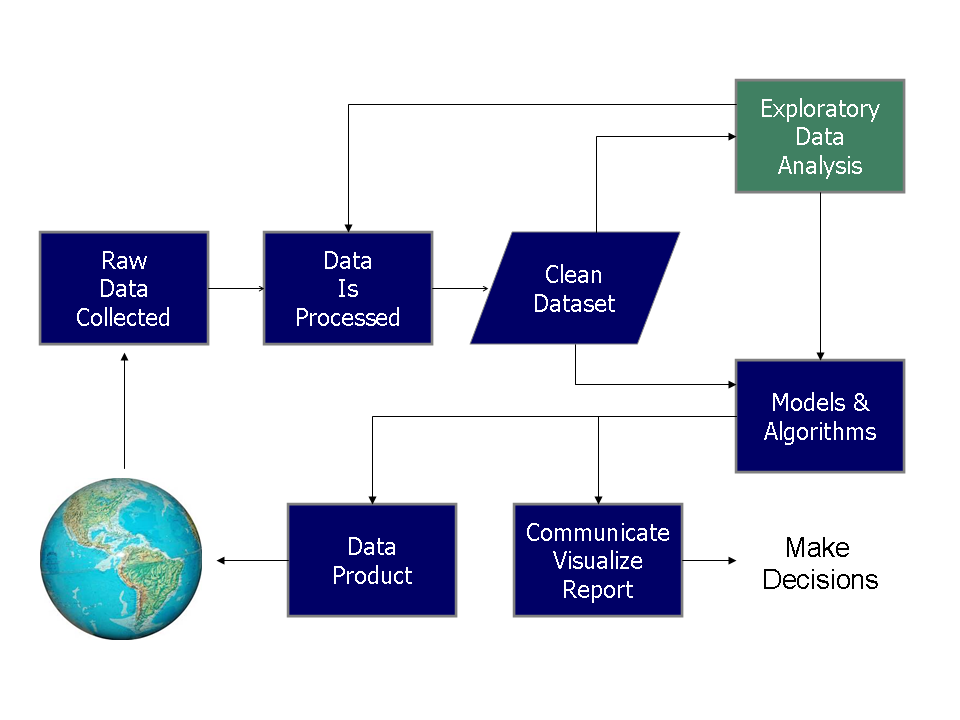
\includegraphics[width = 100mm]{datavisualization.png}
	\caption{La visualizzazione dei dati è un passo fondamentale nell'analisi dei dati.}
	\label{datavisualization}
\end{figure}

